\documentclass[12pt]{article}
\usepackage{graphicx, subfigure, float, amsmath, amssymb, color}
\usepackage[margin = 1.0 in]{geometry}
%\usepackage[style = nature]{biblatex}

% definition of \customlabel, which is used to label supplementary figures and tables
\makeatletter
\newcommand{\customlabel}[2]{%
\protected@write \@auxout {}{\string \newlabel {#1}{{#2}{}}}}
\makeatother



\title{Amino-acid site variability among natural and designed proteins}
\author{Eleisha L.\ Jackson$^1$, Noah Ollikainen$^2$, Arthur W.\ Covert III$^1$,\\ Tanja Kortemme$^{2,3}$, and Claus O.\ Wilke$^1$}
\begin{document}

\date{\today}
\maketitle

\noindent
$^1$ Institute of Cellular and Molecular Biology, Center for Computational Biology and Bioinformatics, and Department of Integrative Biology, The University of Texas at Austin, Austin, Texas, USA\\
$^2$ Graduate Program in Bioinformatics,University of California San Francisco, San Francisco, California, USA\\
$^3$ California Institute for Quantitative Biosciences (QB3) and Department of Bioengineering and Therapeutic Science, University of California San Francisco, San Francisco, California, USA


%Use \textbf{} to bold tetxt
\begin{abstract}
{\color{blue}
Protein structure prediction software attempts to create protein structures that are structurally similar to natural proteins. We examine how accurately Rosetta, a protein prediction software, reconstructs observed patterns of variability found in natural proteins. We use Rosetta to design proteins and then compare these designed proteins with natural proteins. Our comparisons include site variability, observed distributions at sites and the effects of protein structure on site variability. Proteins designed with a fixed backbone underestimate the amount of site variability observed in natural proteins while proteins designed with a flexible backbone result in more site variability. Intermediate flexibility during design results in site variability patterns that most accurately resemble those found in natural proteins. From these results we conclude that intermediate backbone flexibility during design results in more accurate protein design and that scoring functions that determine acceptable substitutions must improve to account for structural constraints on site variability patterns.
}
\end{abstract}


\section{Introduction}
\label{Introduction}

{\color{blue}
There are many selective pressures that affect the rate at which protein sequences change over time. Some of these important determinants include protein dispensability, expression and protein structure. A protein's structure determines how it can function and interact with other proteins.  Therefore a thorough knowledge of the constraints of protein structure on protein evolution is necessary to understand how proteins function. Many proteins need stable native structure to preserve their function. Understanding how proteins function and evolve is of critical importance for the development of proteins with novel functions, advances in drug therapy and increasing our knowledge of disease.  
}

{\color{blue}
It is well documented that protein structure has an influence on variability seen at sites \cite{Franzosa2009, Ramsey2011}. Computational protein design can be used develop and analyze protein structures allowing us to further our knowledge of the effects of protein structure on sequence evolution. In fact recent work using knowledge gained from computational design has resulted in the design of proteins that bind to an influenza virus \cite{Fleishman2011}. During design, protein sequences are optimized for stability \cite{Butterfoss2006, Das2008}. Protein stability has been shown to be an important selective force on proteins \cite{Drummond2008}. Therefore these optimized structures can be used to assess the constraints of structural stability on protein sequences. Comparing designed and natural proteins will allow us to understand how protein structure, and in particular, protein stability shape observed sequence patterns.
}

{\color{blue}
In this paper, we assess the ability of designed proteins to re-capture natural sequence properties by directly measuring variability patterns and comparing them to observed patterns in natural proteins. We not only examine how similar site variability is but we also examine whether the relationships between site position and variability in natural proteins are maintained in designed proteins.  First we obtained a selection of natural proteins and used the design software, Rosetta (http://www.rosettacommons.org/), to design proteins that are structurally similar. We then measured site variability within the natural proteins and compared this variability to the variability within the designed proteins. We also compared the amino acid distributions at sites within natural proteins with that of sites in designed proteins. Lastly we compared how structure constrains sequence variability within both types of proteins (natural and designed). By directly measuring and comparing amino acid patterns of designed proteins with natural proteins, we can determine which properties in natural proteins designed proteins accurately capture. 
}

\section{Methods}
\label{Methods}

\subsection{Data sets}

We analyzed two data sets, one of whole yeast proteins and one of protein domains. The yeast-proteins data set was taken from Ref.\ \cite{Ramsey2011} and comprised 38 protein structures homologous to an open reading frame in \emph{Saccharomyces cerevisiae}. For each of those structures, we had at least 50 homologous natural sequences, also taken from Ref.\ \cite{Ramsey2011}. The protein-domain data set was taken from Ref.\ \cite{OllikainenKortemme} and comprised 40 protein domains {\color{red} a little more detail here}. For each of these protein domains, we obtained alignments of homologous natural sequences from the Pfam database \cite{Pfam}, as described \cite{OllikainenKortemme}.


\subsection{Protein design}

For each structure in both data sets, we computationally designed 500 variants each, using multiple design methods. All design methods we used are implemented in the protein-design software Rosetta \cite{generic-rosetta-reference}. First, we used standard fixed-backbone design \cite{fixed-design}. In this method, the protein backbone remains fixed and only amino-acid side chains are allowed to move. Second, we used the flexible-backbone method Backrub \cite{Smith2008}, which first generates an ensemble of alternative backbones and then designs side chains onto these backbones. The Backrub method takes as input a temperature parameter that determines the extent of backbone movements that occur during design. A temperature of zero corresponds to the fixed-backbone case while a temperature in excess of 1 allows substantial backbone movements. Here, we used temperatures spanning from 0.03 to 2.4. For the protein-domain data set, we also carried out one additional design method, called ``Soft''. In this method, {\color{red}which is more similar to a fixed-design method but allows for minor backbone movements, \textbf{(correct?)}} the energy function used during sequence design dampens the weight of the repulsive Lennard-Jones (LJ) potential term. {\color{red}Do we have a reference for the ``soft'' design method?}

{\color{red}Is the following sentence correct? ``We used MUSCLE \cite{Edgar2004} to align our designed sequences.'' Aligning designed sequences is wrong, and they should be automatically aligned anyway.}

Protein designs for the protein-domain data set have been previously published \cite{OllikainenKortemme}, while the designs for the yeast-proteins data set where newly generated for the present study.

\subsection{Data analysis}

We quantified the variability of sites in amino-acid alignments using site entropy $H_i$, defined as $H_i=\sum_{j}p_{ij}\ln p_{ij}$. Here, $p_{ij}$ is frequency of amino acid $j$ in alignment column $i$, and the sum runs over all amino acids. {\color{red}Did we do a correction for zero counts? Maybe we should not.}

We compared amino-acid distributions of designed sequences to those of natural sequences using the Kullback-Leibler (KL) divergence. The KL divergence $D^\text{KL}_i$ is defined as $D^\text{KL}_i= \sum_j  p_{ij} \ln  (p_{ij}/q_{ij})$, where $q_{ij}$ is the frequency of amino acid $j$ in column $i$ of the reference alignment, and $p_{ij}$ is the corresponding frequency in the alignment that is being compared to the reference alignment. The sum runs over all amino acids. The KL divergence is inherently an asymmetric distance measure, comparing a probability distribution of interest to a reference distribution. Unless noted otherwise, we always used natural sequence alignments to calculate the reference frequencies $q_{ij}$ and designed sequence alignments to calculate the frequencies $p_{ij}$. Throughout this work, we calculated $D^\text{KL}_i$ separately at each site $i$ in a protein, and then averaged the $D^\text{KL}_i$ values for all sites in a protein to obtain a mean KL divergence for that protein.

We calculated Relative Solvent Accessibility (RSA) of residues by first calculating the absolute Solvent Accessibility (SA) for each residue, using the software DSSP \cite{Kabsch1983}. For each protein, we extracted the chain of interest from the PDB structure and ran DSSP only on that chain. We calculated RSA by dividing the SA value for each residue by the maximum possible SA value, as given in Ref.\ \cite{Tien}. 

\section{Results}
\label{Results}


We wanted to assess the extent to which the sequence space of computationally designed proteins overlaps with the sequence space occupied by homologous natural proteins. Our general approach was to compare alignments of designed protein sequences to alignments of homologous natural sequences, for approximately 80 distinct protein structures. For each structure, we considered several different design methods (see Methods for details), and we designed 500 {\color{red}(Is this correct for Noah's data set?)} sequences for each structure and method. The protein structures we considered were subdivided into two distinct data sets, a data set of 38 yeast protein structures previously analyzed in Ref.\ \cite{Ramsey2011} and a data set of 40 protein domains previously analyzed in  Ref.\ \cite{OllikainenKortemme}. Throughout this study, we analyzed these two data sets separately, because they corresponded to structures of substantially different sizes. The mean number of amino acids per structure was 215.4 in the yeast-proteins data set and 86.1 in the protein-domains data set.

\subsection{Overall site variability}
\label{SiteVariability}

We first compared overall amino-acid variability in designed and natural proteins. We assessed amino-acid variability at individual sites by calculating the entropy $H_i$ at each site $i$ in alignments of either designed or natural proteins. We then calculated the mean entropy over all sites in each alignment and used that quantitiy as a measure of the overall amino-acid variability in the alignment.

We found that protein design using a fixed backbone generally yielded insufficient site variability compared to natural sequences (Fig. \ref{MeanEntropyComparison}). The most variable proteins under fixed-backbone design showed only about as much variability as the least variable natural proteins. Overall, there was a significant shift towards higher variability in natural proteins relative to proteins designed with fixed backbone (paired $t$ test, {\color{red}$P=\dots$} for the yeast-proteins data set and {\color{red}$P=\dots$} for the protein-domain data set). When switching from fixed-backbone design to variable-backbone design, we found that overall site variability increased. Further, site variability increased monotonously with the degree of backbone flexibility allowed during design, as measured by the design temperature (Fig. \ref{MeanEntropyComparison}). At the highest temperatures, site variability in designed proteins consistently exceeded that of natural proteins. Proteins designed at intermediate temperatures of 0.6-0.9 had site variability that mostly closely resembled that of natural proteins. However, at those temperatures, natural proteins generally showed a larger spread in variabilities than designed proteins did (Brown–Forsythe test for equal variances, {\color{red}$P=\dots$} for the yeast-proteins data set and {\color{red}$P=\dots$} for the protein-domain data set).



\subsection{Amino-acid distributions}
\label{AminoAcidDistributions}

We next compared amino-acid distributions between designed and natural sequences. First we looked at overall amino acid frequencies. We found that by-and-large, amino acid frequencies in designed proteins mirrored those in natural proteins (Figs.~\ref{AAFreqsYeastProteins} and \ref{AAFreqsProteinDomains}). The biggest differences arose in Cys, Pro, His, Trp, Phe, Ala. Overall, we observed that hydrophobic residues tended to be under-represented in designed proteins whereas hydrophilic residues tended to be over-represented. This trend was stronger in the protein core than on the surface (Figs.~\ref{AAFreqsYeastProteins} and \ref{AAFreqsProteinDomains}). We also observed that the longer proteins in the yeast-proteins data set showed larger deviations between designed and natural sequences than the shorter proteins in the protein-domains data set. Finally, when comparing different design methods and design temperatures, we found that differences in amino-acid distributions were relatively minor (not shown).

Even if overall amino-acid distributions are approximately correct, the amino-acid distributions at individual sites can be poorly predicted \cite{Ramsey2011}. Therefore, we next compared, separately at each site, the similarity between amino-acid distributions in natural proteins and those in designed proteins. To carry out this comparison, we employed the Kullback-Leibler (KL) divergence {\color{red}ref?}, which measures how similar one probability distribution is to a reference distribution. A KL divergence of zero implies that the distributions are identical. The higher the KL divergence, the more dissimilar the focal distribution is to the reference distribution. (Note that KL divergence is not symmetric: if we swap the focal and the reference distribution, we will generally obtain a different KL divergence value.) We calculated the KL divergence at each site in each protein, and then averaged over sites within a protein to obtain a mean similarity score for each protein. As a control, we also randomly split the alignment of natural sequences for each protein structure into two halves and calculated the mean KL divergence of natural sequences against themselves.

First, in all comparisons, we found that the KL divergence of designed relative to natural sequences was much bigger than the KL divergence of natural sequences relative to themselves (Figs.~\ref{AADisFig1} and~\ref{NoahAADisFig1}). This finding indicates a substantial discrepancy between designed and natural sequences at individual sites. Second, we found that the mean KL divergence decreased with increasing design temperature (Figs.~\ref{AADisFig1}A and~\ref{NoahAADisFig1}A). Thus, according to the KL divergence measure, structures designed with the most flexible backbones had the most similar amino-acid distributions to those found in natural sequences.

However, the result that sequences designed at the highest temperatures are the most similar to natural sequences may be an artifact of the KL divergence measure. As design temperature increases, amino-acid variability increases, and amino-acid distributions become more uniform. A more uniform distribution is generally going to display more overlap with any given distribution than a more localized distribution, if the localized distribution is not correct. Thus, the decrease in KL divergence with increasing temperature may simply reflect the broadening of the distribution, not an actual improvement in reproducing natural amino-acid distributions. To assess whether amino-acid distributions in designed sequences were simply broadening with increasing temperature, or whether they were actually converging on the natural distributions, we carried out a second set of comparisons. We rank-ordered amino acids by frequency at each site in each protein, and then calculated the KL divergence of the rank-ordered distributions. This comparison considers only the shape of the distribution and does not assess whether the correct amino acids are present at individual sites. This second comparison generally found much lower KL divergence levels, even though still not as low as what was found for the control comparison of natural sequences with themselves (Figs.~\ref{AADisFig1}B and~\ref{NoahAADisFig1}B). More importantly, now KL divergence reached a minimum around a temperature of 0.6
(yeast proteins, Fig.~\ref{AADisFig1}B) to 0.9 (protein domains, Fig.~\ref{NoahAADisFig1}B) and rose again beyond that value. This finding indicates that higher design temperatures do not unequivocally produce more natural amino-acid distributions. Instead, there is an intermediate temperature, approximately coinciding with the temperature at which overall sequence variability matches best, at which amino acid distributions also are most similar.

\subsection{Site variability and solvent accessibility}
\label{ProteinStructure}

The previous analyses demonstrated that while designed proteins overall look similar to natural proteins, there are also important differences. We next wanted to identify whether these differences were present uniformly throughout the structure or could be located to specific structural regions. In our analysis of amino-acid distributions, we had already seen that amino-acid distributions seemed to deviate more at buried sites than at exposed sites (Figs.~\ref{AAFreqsYeastProteins} and~\ref{AAFreqsProteinDomains}).

We first plotted site variability against relative solvent accessibility (RSA, a dimensionless number from 0 to 1 measuring the relative solvent exposure of individual residues) for individual proteins. 


{\color{blue}
We wanted to determine how protein structure constrains protein sequence variability using Rosetta. In particular we were interested in how closely the designed proteins captured the relationship between structure and sequence variability within natural proteins. The Relative Solvent Accessibility (RSA) of a site quantifies how buried a residue is within the protein's core \cite{Franzosa2009}.  A lower RSA value means a residue is more buried. By correlating the RSA value of a site with its entropy we can examine the relationship between structure and site variability (as measured by entropy).  On average within the natural proteins there was a higher correlation between entropy and RSA at sites (Figure \ref{StructureFig1}A, \ref{NoahStructureFig1}A) as compared to the designed. This means that sites on the surface of a protein experience greater site variability compared to sites within the protein's core. In addition, proteins with a higher correlation between RSA and entropy in the natural proteins have a higher correlation in the designed proteins (Figure \ref{StructureFig1}B, \ref{NoahStructureFig1}B). However, designed proteins did not perfectly capture the relationship between structure and site variability. 

Overall the designed proteins have a lower correlation between RSA and entropy.  In general, the fixed backbone treatment resulted in a lower correlation between entropy and RSA at sites suggesting there were not enough substitutions made on the surface.  This applied to both fixed backbone methods. Among the designed proteins, intermediate temperatures had a higher correlation between entropy and RSA at sites. For example in the dataset comprised of 40 proteins, temperatures of 0.03, 0.1, 0.3 the median correlation was approximately 0.20, the highest of any of the designed. As the backbone became more flexible more amino acid substitutions were allowed in general - core or surface. In fact, as the temperature increased past 0.9 for some sites we observed a negative correlation between RSA and entropy.  This resulting lower correlation between RSA and entropy suggests there were more substitutions that were allowed within the core of the protein. Therefore within natural proteins there was a stronger correlation between structure and site variability.  To test this, we calculated the correlation between RSA and correlation between sites using different temperature values in an attempt to recover the correlation seen in natural proteins. For this analysis, we used a lower temperature (0.3) for buried sites and a higher temperature (0.6 and 0.9) for surface sites. These temperatures were chosen because these temperatures mostly closely replicated the site variability seen in buried and surface sites. During this analysis, we found that when different temperatures are used for the buried and surface sites are used, the correlation between RSA and entropy at sites is similar to that seen in natural proteins (Figs.~\ref{Mixed_RSA_Entropy_Duncan} and~\ref{Mixed_RSA_Entropy_Noah}). This means that surface sites and buried sites have two different optimal design temperatures for replicating site variability seen in natural sites. 




Next we more closely examined how RSA affected the amino acid distributions at sites with both the natural and designed proteins. At each site within our protein alignments amino acids were ranked, k = 0,1,..., 20 corresponding to how frequent they were found at that site. Amino acid frequencies were found to be proportional to an exponential, $\exp (-\lambda k)$ as discovered in previous work \cite{Ramsey2011}. We used Maximum Likelihood Analysis (MLE) to fit the parameter $\lambda$ as a linear function of RSA in the form $$ \lambda = a \text{RSA} + b $$ $\lambda$ describes the shape of the amino acid distribution at site. A large $\lambda$ describes a distribution that is more skewed. A site with a large lambda means that often times there are only a few types amino acids that are observed at that site. The intercept, $b$, determines how much sequence variability is independent of RSA. A larger intercept means a larger $\lambda$, which leads to less variability. The slope, $a$, determines how much influence RSA has on $\lambda$. A slope of zero for a single protein means there is no difference between core and the surface amino acid distributions in that protein. Comparing the slopes and intercepts of the natural protein with the designed proteins allowed us understand how protein structure and site variability differ between the two different classes of proteins. 

Proteins designed with fixed backbones have intercept values that are most similar to natural proteins. Designed proteins with a flexible backbone have lower intercepts (Figure \ref{StructureFig3}B, \ref{NoahStructureFig3}B). In the natural proteins, most proteins had a negative slope. This means that there was less sequence variability at sites within the core when compared to sites on the surface.  On average the designed proteins had a larger slope than natural proteins (Figures \ref{StructureFig3}A, \ref{NoahStructureFig3}A) . In addition, as the temperature increased, the slope shifted and increased. This means that increasing temperature caused sites to exhibit more to be more site variability. The slope was positive because more mutations were allowed in the core protein. We conclude that proteins that are designed fail to accurately capture the restriction of acceptable amino acids within the protein core. 


In order to examine whether there was a difference in the mean entropy of sites in the core of the protein and those on the surface we calculated the mean entropy for sites according to how buried they were. Sites were classified as either buried, partially buried, and or exposed if they had an RSA value of less than 0.05, a value between 0.05 and 0.25 inclusive, and a value greater than 0.25 respectively. Both buried and partially buried sites exhibited trends similar to those observed when you compare the mean values of all sites. For example, for buried residues within the first dataset of 38 whole proteins, a temperature of 0.6 is optimal. However, within these same proteins, surface sites have a optimal temperature of 0.9 (Figure \ref{Duncan_Position_Entropy}). Therefore in order to capture the site variability that is seen at surface sites, one has to design proteins with a more flexible backbone compared to that used for buried sites if you want to recover the site variability seen in natural proteins. The amount of site variability tells us nothing about whether the types of amino acids found at each site were similar. For insight we investigated the amino acid distributions at sites within the two types of proteins for similarities and dissimilarities. 
}


\section{Discussion}

{\color{blue}
We designed a series of proteins from 38 natural yeast proteins. These designed proteins were used to create a series of alignments that we compared to natural alignments. These natural alignments were created using sequences that were homologous to the natural proteins used in the designed process.  We compared site variability as measured by entropy between the designed and natural proteins. Proteins that were designed with a backbone with intermediate flexibility exhibited site variability similar to sites within natural proteins. In addition, these proteins also had amino acid distributions at sites that are most similar in shape to sites within natural proteins. This suggests that not only do these proteins exhibit appropriate levels of site variability but they also more are accurate at using similar types of amino acids at those sites.  Lastly we used relative solvent accessibility to determine the effects of protein structure on site variability patterns in natural proteins. After measuring the effects of protein structure in natural proteins, we compared this effect to that of protein structure on designed proteins. 

Designed proteins appear to do a less accurate job at capturing the type of constraints that structure has on amino acid patterns at sites within natural proteins. According to our analysis, natural proteins had a much higher correlation between RSA and site variability. In natural proteins site variability is more strongly influenced by the site's position within the protein. In these proteins there is a much greater difference between the variability experienced by proteins on the surface of the protein and the variability experienced by sites with the proteins core. Designed proteins do not capture this difference.  Our results could help improve current software capabilities. The inability of Rosetta to accurately capture site variability differences between the core and the surface point to the need for improvements in determining scoring whether substitution should be made at a site. Improvements in the scoring functions of substitutions might lead to more accurately designed proteins in the future.
}

\bibliographystyle{plain} %"style
\bibliography{ProjectBib} %expected file "my refs.bib"

\cleardoublepage

\section{Figures}

%Figure 1
\begin{figure}[H]
%\centering
\centerline{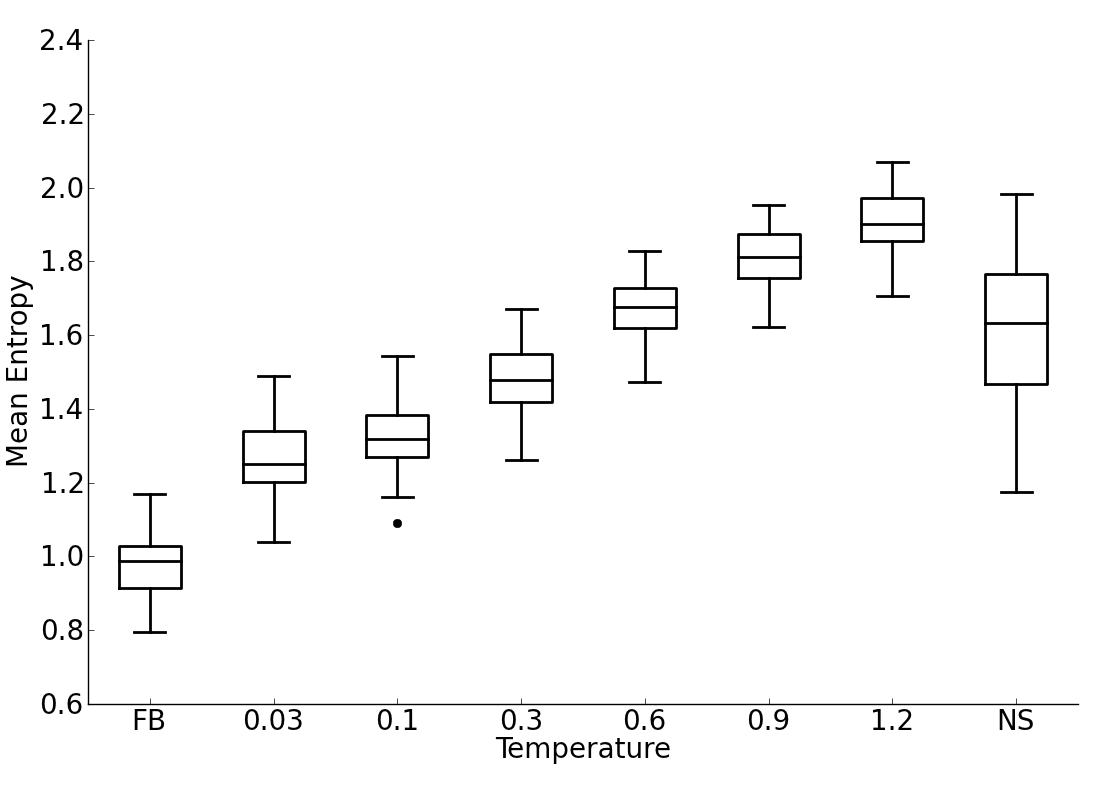
\includegraphics[width = 3in]{figures/Mean_Entropy_vs_Temp_Boxplot.png}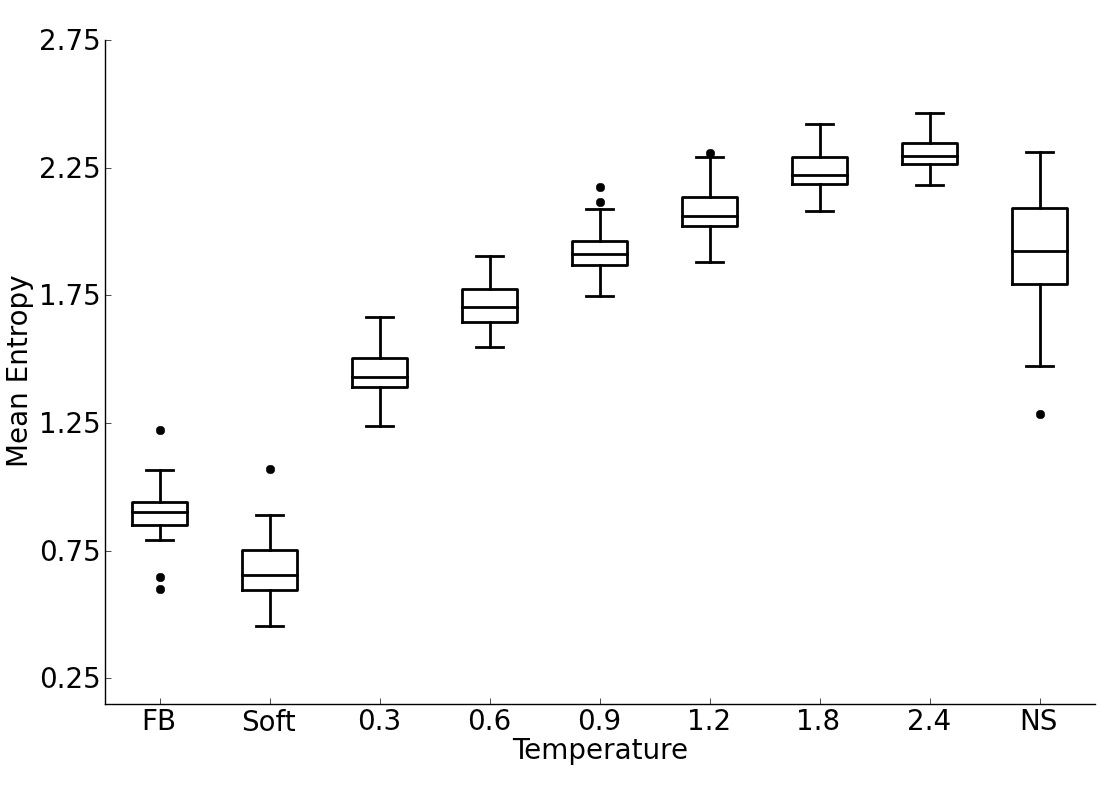
\includegraphics[width = 3in]{figures/Mean_Entropy_vs_Temp_Boxplot_Noah.png}}
\caption{Mean site entropy for designed and natural proteins. Each boxplot represents the distribution of mean site entropies within the respective dataset (left: yeast proteins; right: protein domains). ``FB'' refers to fixed-backbone design. Temperature values refer to the design temperature used during the Backrub design method. ``NS'' refers to natural sequences. ``Soft'' refers to the Soft design method. We find generally that more flexible backbones during desing allow for more site variability. Intermediate temperatures (0.6-0.9) produce site variabilities most similar to those seen in natural sequences. Overall, natural sequences in the protein-domains data set are more variable than are those in the yeast-proteins data set. {\color{red}The two figures need to be combined into one, labeled with "A" and "B", and put on the same $y$ scale.}}
\label{MeanEntropyComparison}
\end{figure}


\begin{figure}[H]
\centerline{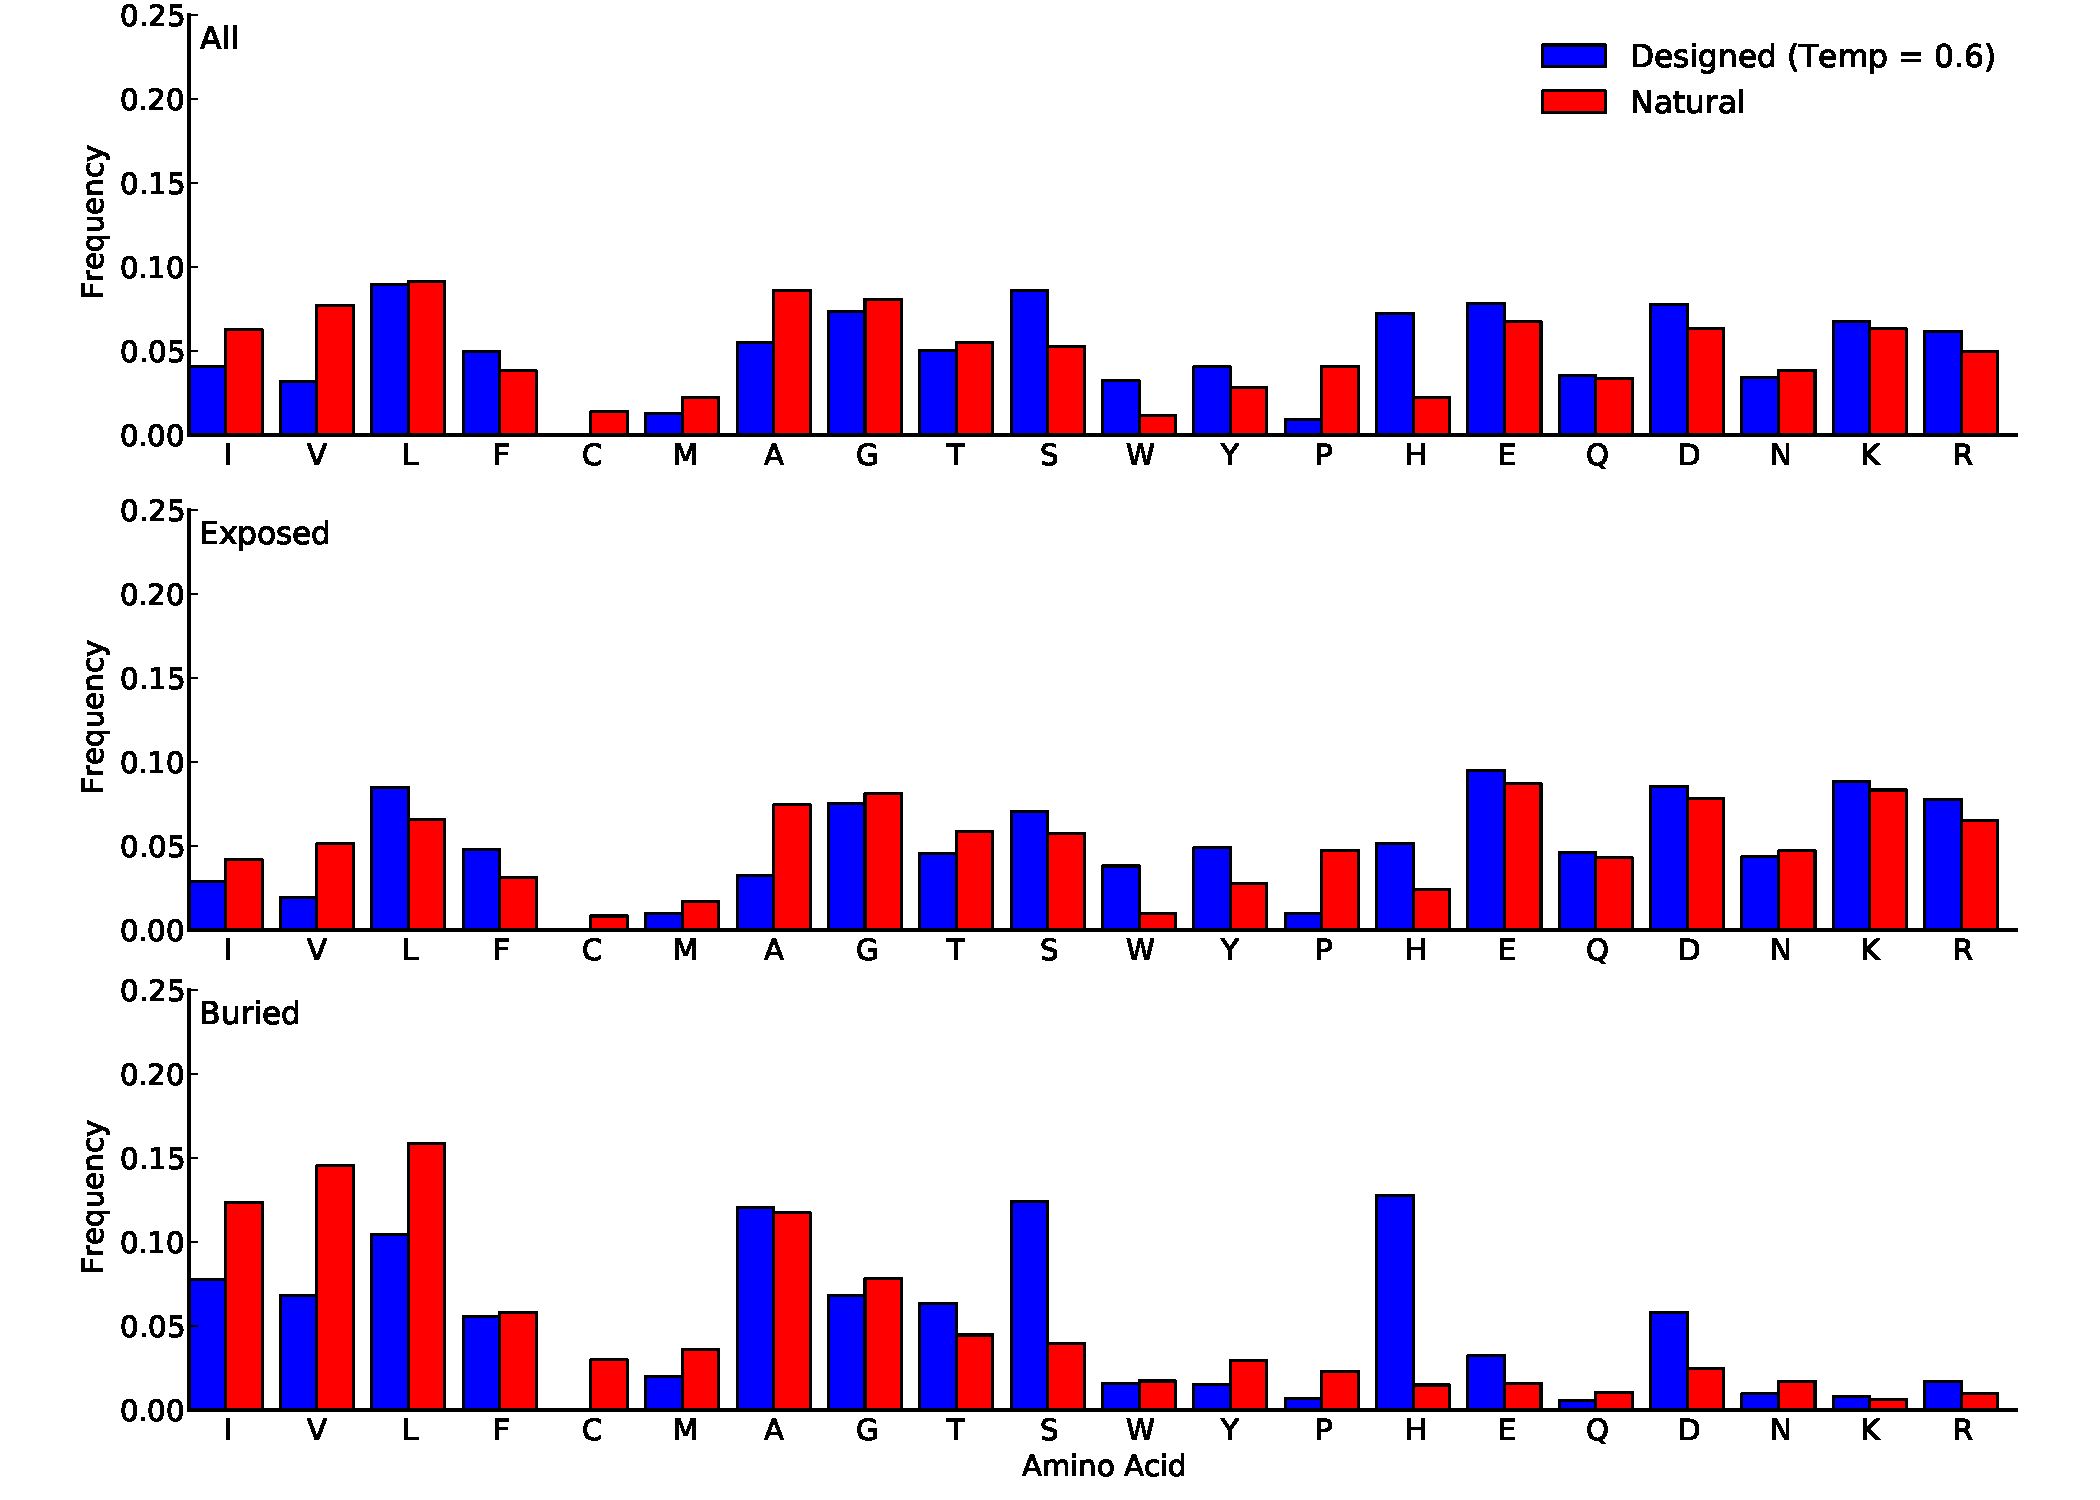
\includegraphics[width = 5in]{figures/Duncan_Freq_Combo_Plots_06.pdf}}
\caption{Amino-acid frequencies in designed and natural proteins. Frequencies were calculated over all sites in all proteins belonging to the yeast-proteins data set. For designed proteins, only flexible-backbone designs with design temperature 0.6 were considered. Top: overall frequencies. Middle: frequencies at exposed sites (defined as sites with $\text{RSA}>0.05$). Bottom: frequencies at buried sites (defined as sites with $\text{RSA}\leq0.05$).}
\label{AAFreqsYeastProteins}
\end{figure}


\begin{figure}[H]
\centerline{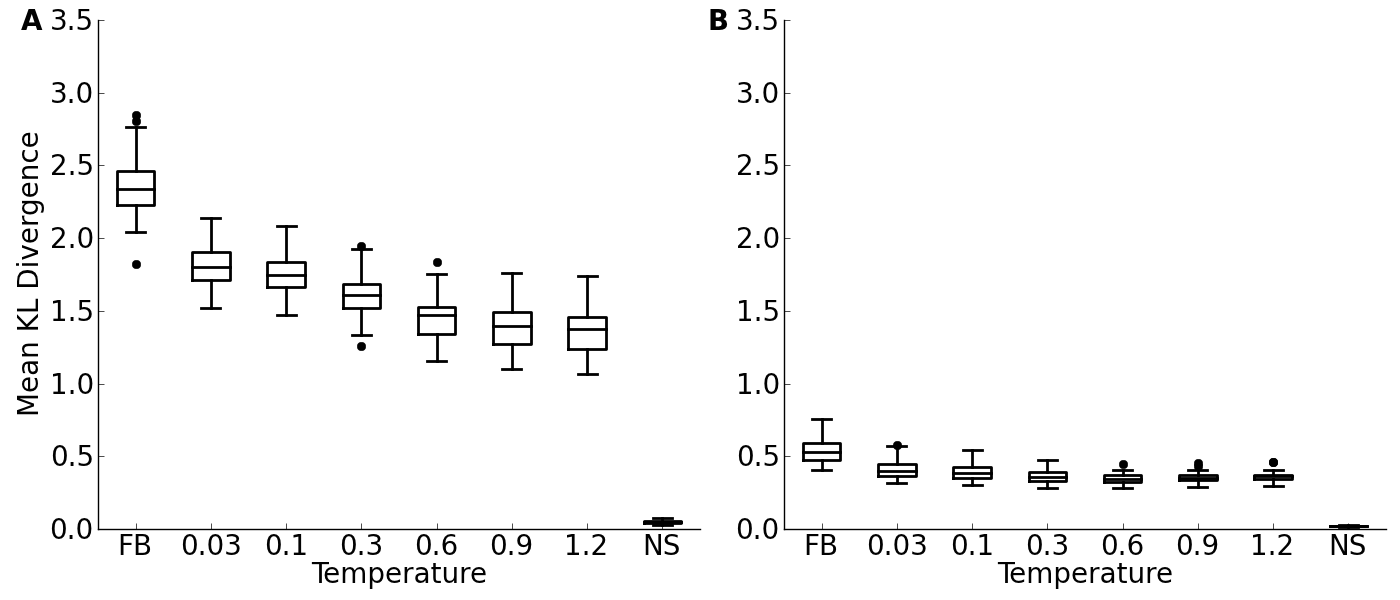
\includegraphics[width = 6in]{figures/Mean_KL_vs_Temp_Boxplot.png}}
\caption{Mean Kullback-Leibler (KL) divergence for designed and natural proteins, shown for the yeast-proteins data set. A higher KL divergence indicates that the amino-acid distributions at sites in designed proteins are less similar to the corresponding distributions in the natural proteins. ``FB'' refers to fixed backbone design, and ``NS'' refers to the control case where natural sequences are compared to themselves. (A) KL divergence calculated from the relative frequencies of the 20 amino acids. (B) KL divergence calculated from rank-ordered frequency distributions. The most common amino aicd in the reference distribution is compared to the most common amino acid in the focal distribution, the same is done for the second-most common amino acid, and so on, irrespective of the type of amino acids.}
\label{AADisFig1}
\end{figure}


\cleardoublepage

\section{Supporting Figures}

\centerline{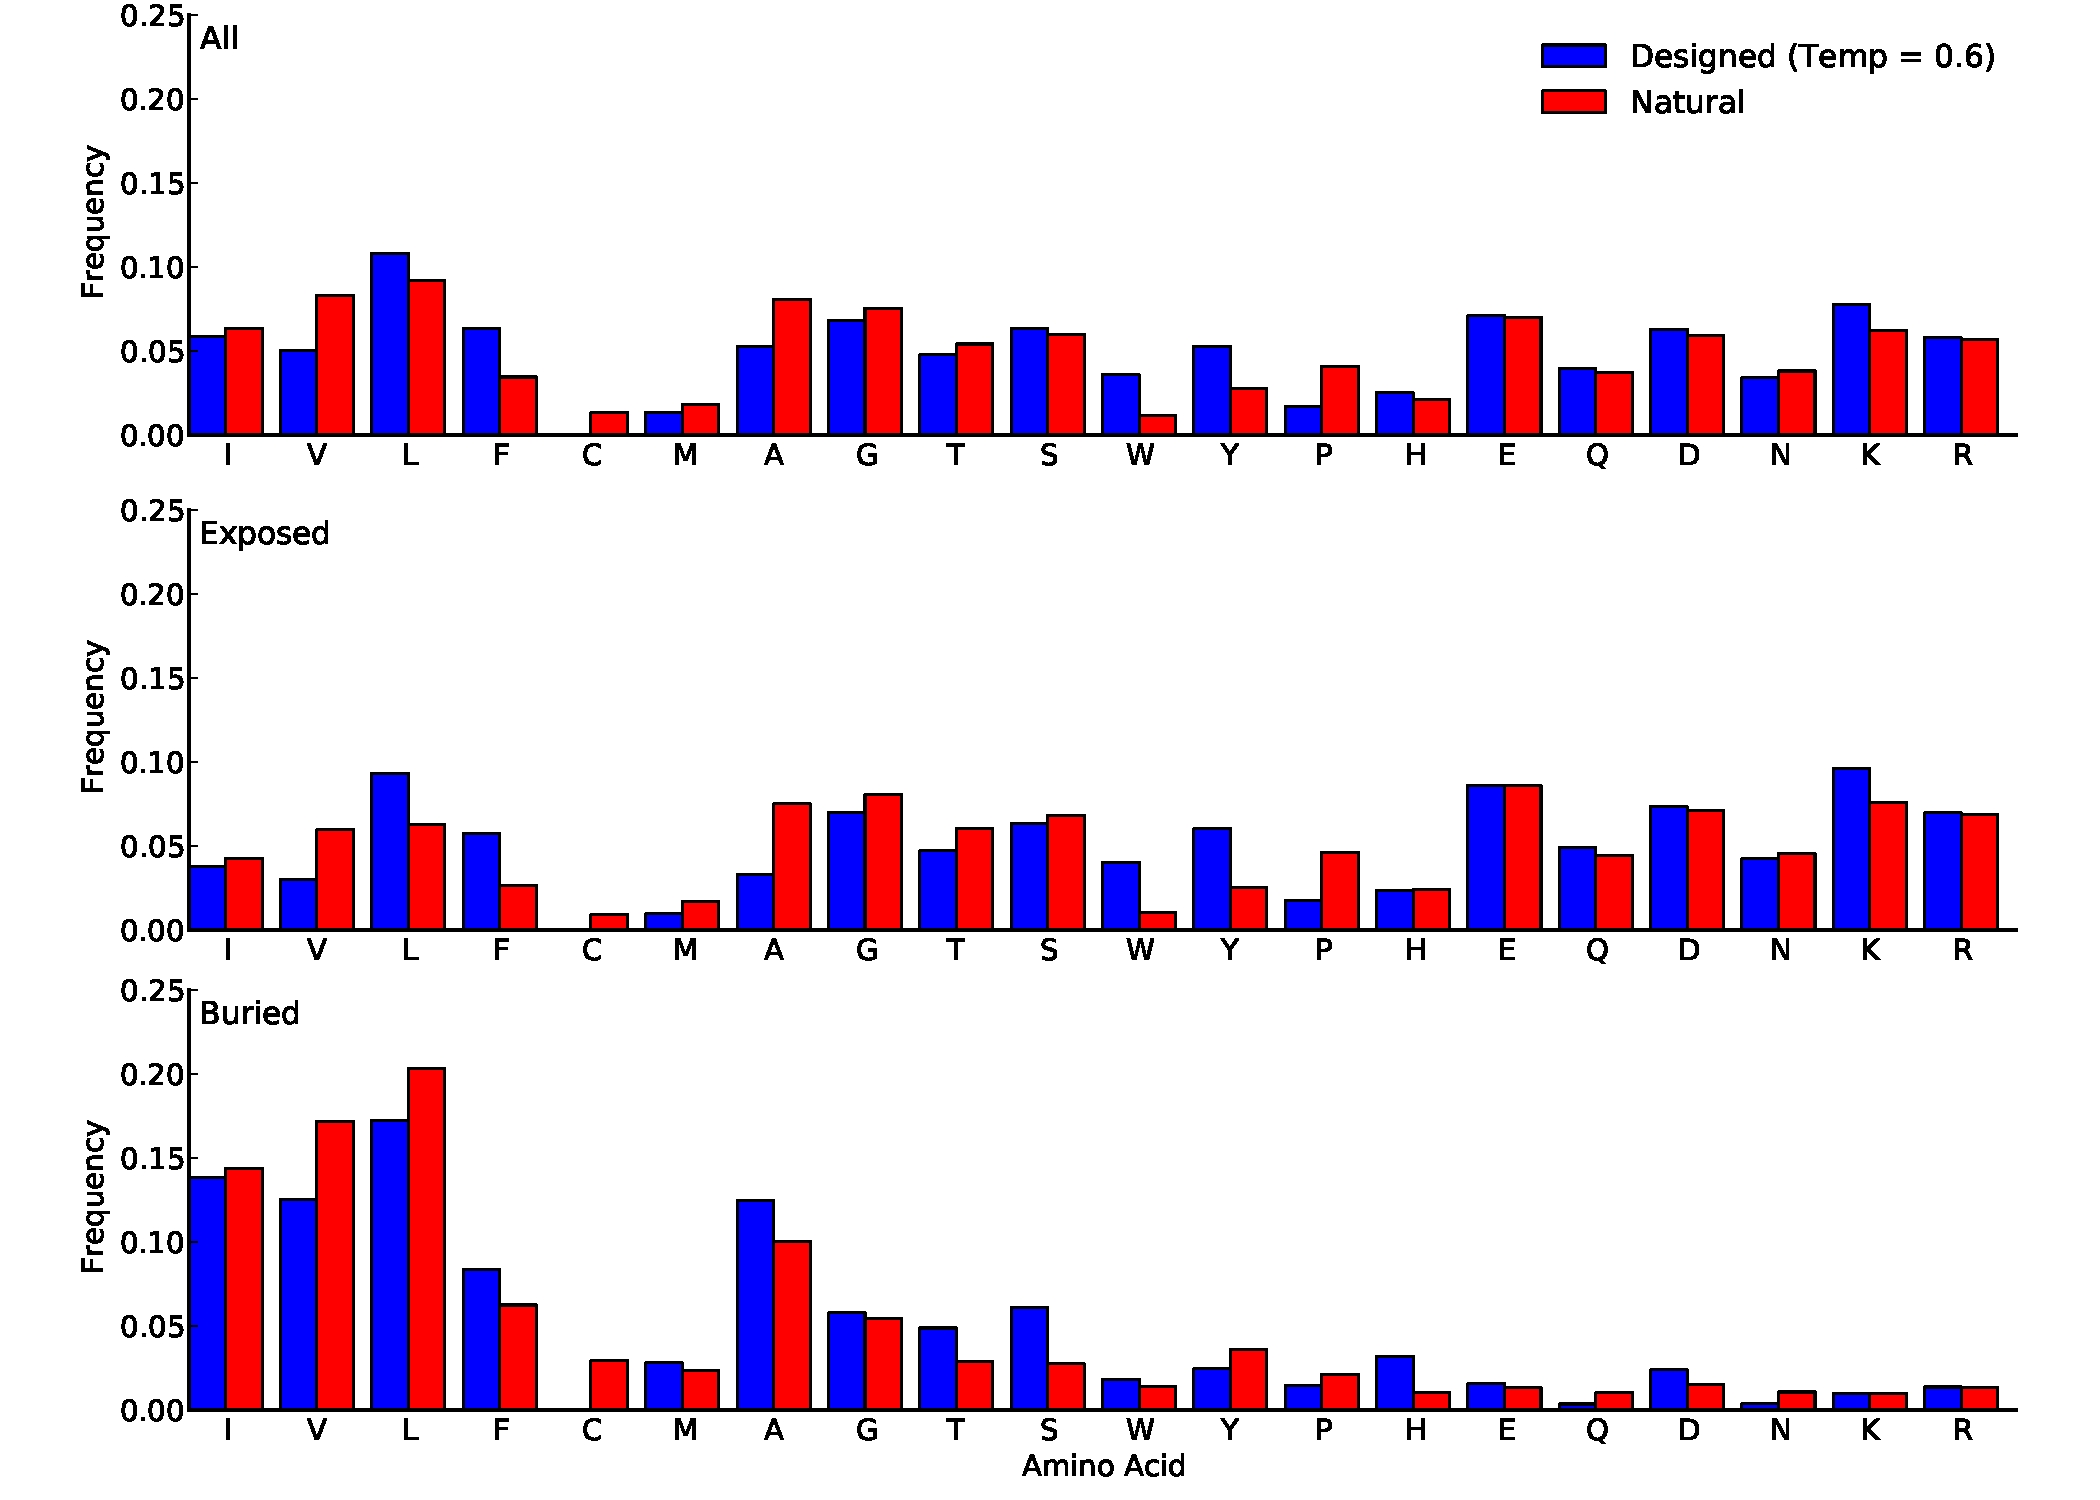
\includegraphics[width = 5in]{figures/Noah_Freq_Combo_Plots_06.pdf}}

\noindent Figure S1. Amino-acid frequencies in designed and natural proteins. Frequencies were calculated over all sites in all proteins belonging to the protein-domains data set. For designed proteins, only flexible-backbone designs with design temperature 0.6 were considered. Top: overall frequencies. Middle: frequencies at exposed sites (defined as sites with $\text{RSA}>0.05$). Bottom: frequencies at buried sites (defined as sites with $\text{RSA}\leq0.05$).

\customlabel{AAFreqsProteinDomains}{S1}

\centerline{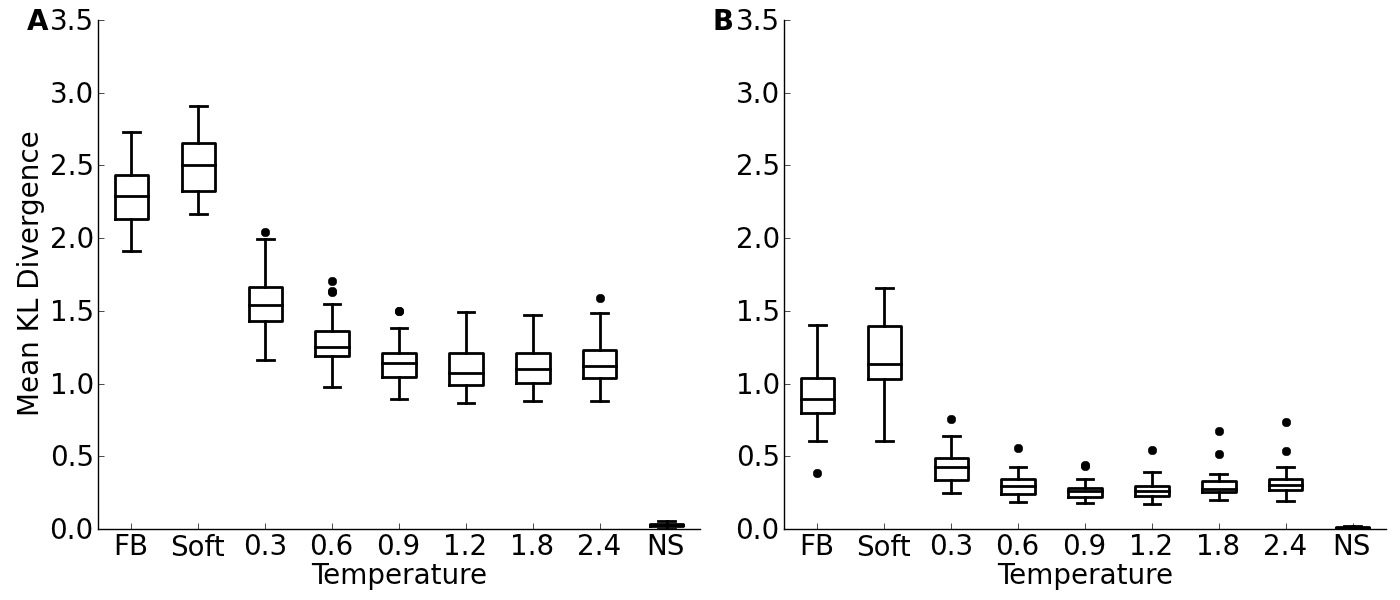
\includegraphics[width = 6in]{figures/Mean_KL_vs_Temp_Boxplot_Noah.png}}
\noindent Figure S2. Mean Kullback-Leibler (KL) divergence for designed and natural proteins, shown for the yeast-proteins data set. A higher KL divergence indicates that the amino-acid distributions at sites in designed proteins are less similar to the corresponding distributions in the natural proteins. ``FB'' refers to fixed backbone design, and ``NS'' refers to the control case where natural sequences are compared to themselves. (A) KL divergence calculated from the relative frequencies of the 20 amino acids. (B) KL divergence calculated from rank-ordered frequency distributions. The most common amino aicd in the reference distribution is compared to the most common amino acid in the focal distribution, the same is done for the second-most common amino acid, and so on, irrespective of the type of amino acids.

\customlabel{NoahAADisFig1}{S2}


\cleardoublepage

\section{Other Figures}


%Figure 12
\begin{figure}[H]
%\centering
%\centerline{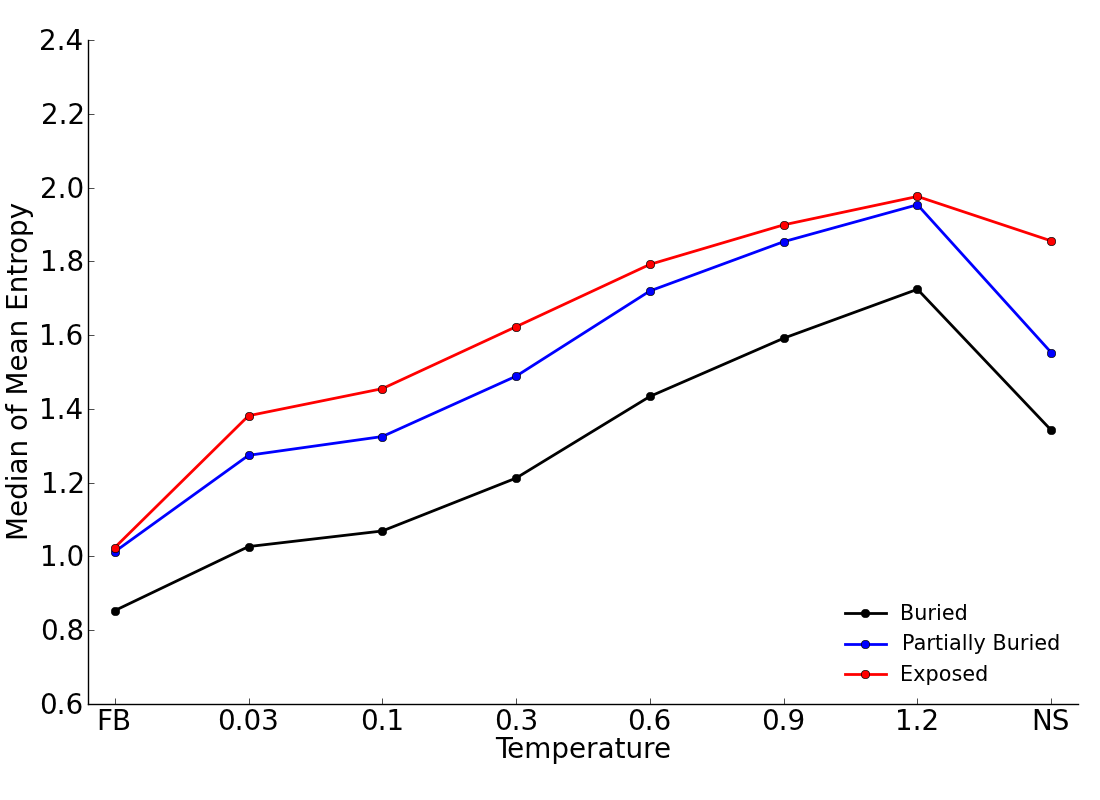
\includegraphics[width = 6in]{figures/Mean_Entropy_Position_Lineplot.png}}
\caption{Median of Mean Entropy versus Temperature sites within series of designed proteins.  Sites are classified as buried, partially buried, or exposed based on RSA magnitude. The temperature refers to the temperature used during the designed process. Higher temperatures allowed for more backbone flexibility. FB and NS refer to the fixed backbone designed proteins and natural proteins respectively.}
\label{Duncan_Position_Entropy}
\end{figure}
 


%Figure 4
\begin{figure}[H]
\centering
%\centerline{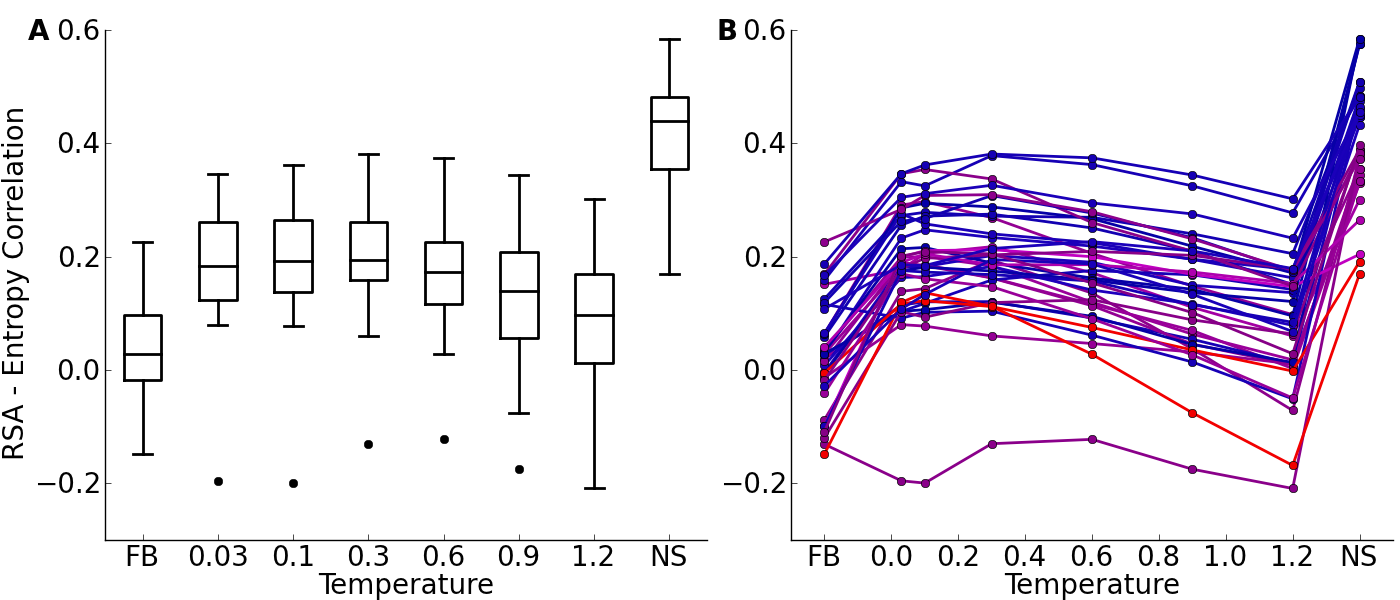
\includegraphics[width = 6in]{figures/Cor_Mean_Entropy_RSA_Combination_Plot.png}}
\caption{Correlation between Entropy and RSA for sites within proteins.  The temperatures represent alignments of designed proteins where an increased temperature relates to an increase level of backbone flexibility during the design process. A) Boxplots of the correlation between RSA and site entropy for various protein alignments. B) Lineplots of the correlation between RSA and site entropy for various protein alignments. The colors correspond to the value of the strength of the correlation between entropy and RSA at sites. Natural proteins have a higher correlation between RSA and entropy at sites.}
\label{StructureFig1}
\end{figure}

%Figure 25
\begin{figure}[H]
%\centering
%\centerline{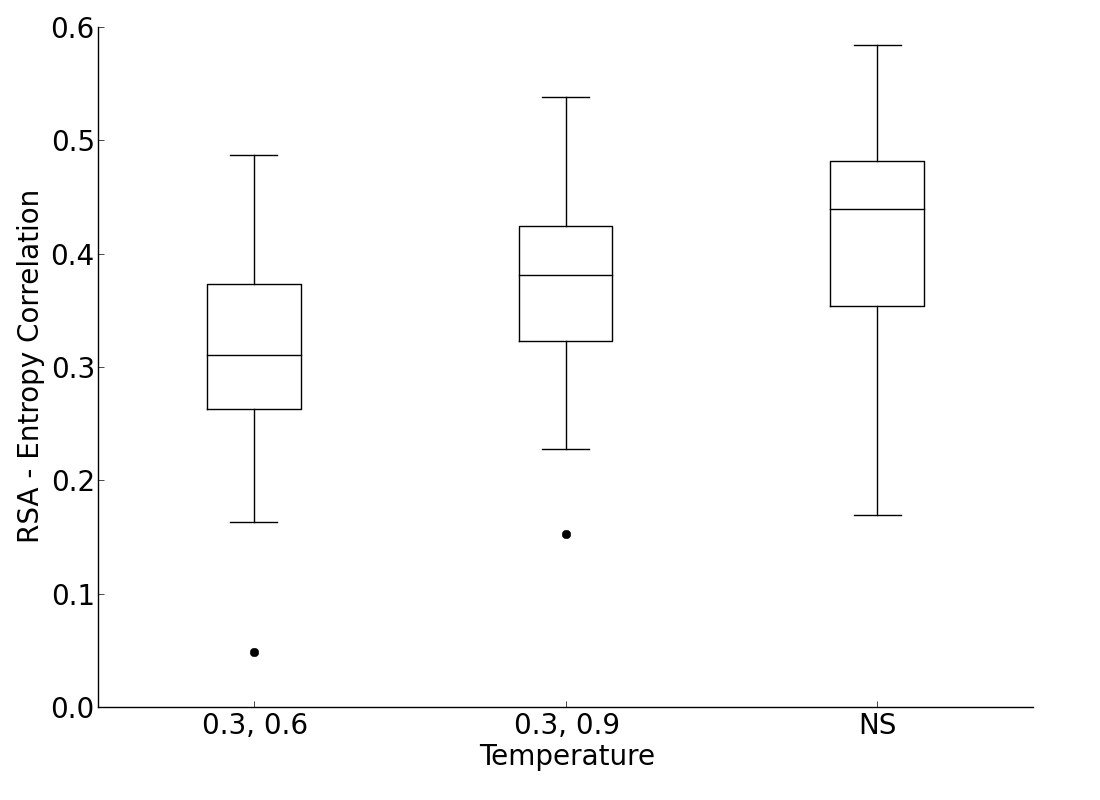
\includegraphics[width = 6in]{figures/Duncan_Mixed_Temp_Correlation_Plot.png}}
\caption{Correlation between RSA and Entropy between entropy at sites for 38 proteins. For each site we classified the site as buried if it had an RSA of than 0.05. All sites not classified as buried are classified as exposed. For sites that were buried, we used the frequencies from the T = 0.3 designed proteins. For the exposed sites we used either the entropy values from T = 0.6 or T = 0.9. By using the different temperature values for each type of site, the correlation between RSA and entropy of sites with the mixed entropy values were to that of the natural proteins.}
\label{Mixed_RSA_Entropy_Duncan}
\end{figure}

%Figure 25
\begin{figure}[H]
%\centering
%\centerline{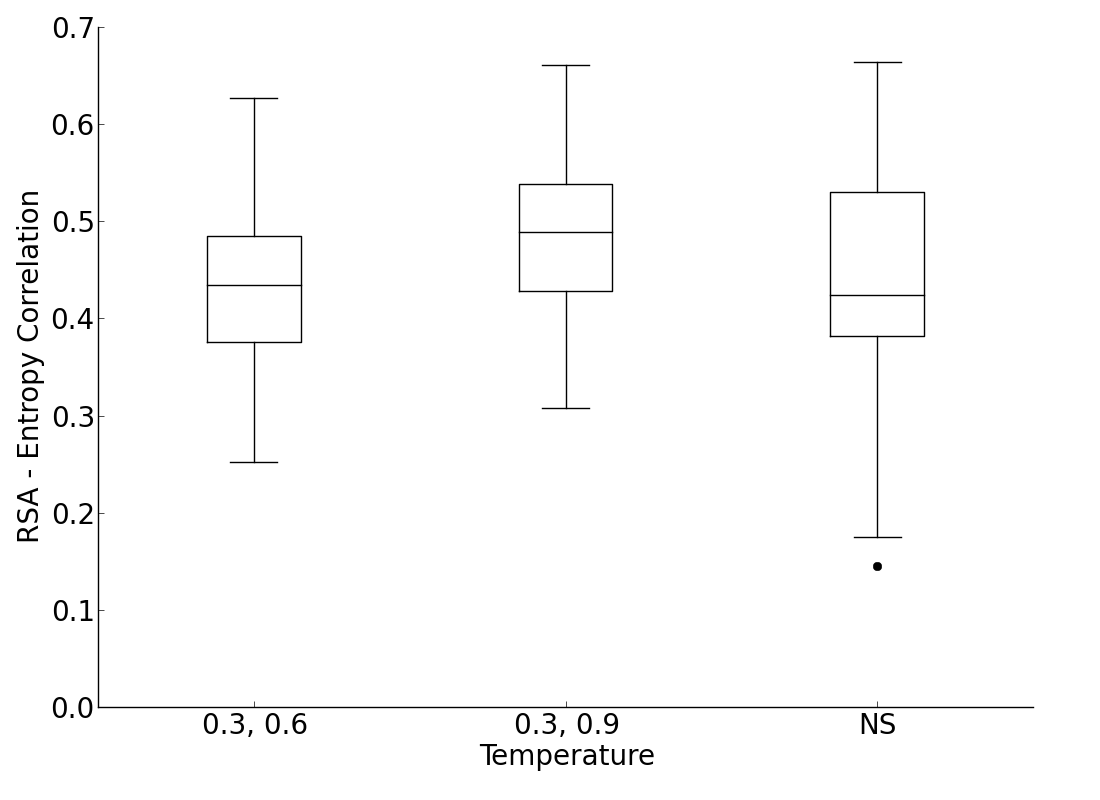
\includegraphics[width = 6in]{figures/Noah_Mixed_Temp_Correlation_Plot.png}}
\caption{Correlation between RSA and Entropy between entropy at sites for 40 protein domains. For each site we classified the site as buried if it had an RSA of than 0.05. All sites not classified as buried are classified as exposed. For sites that were buried, we used the frequencies from the T = 0.3 designed proteins. For the exposed sites we used either the entropy values from T = 0.6 or T = 0.9. By using the different temperature values for each type of site, the correlation between RSA and entropy of sites with the mixed entropy values were to that of the natural proteins.}
\label{Mixed_RSA_Entropy_Noah}
\end{figure}

%Figure 5
\begin{figure}[H]
\centering
%\centerline{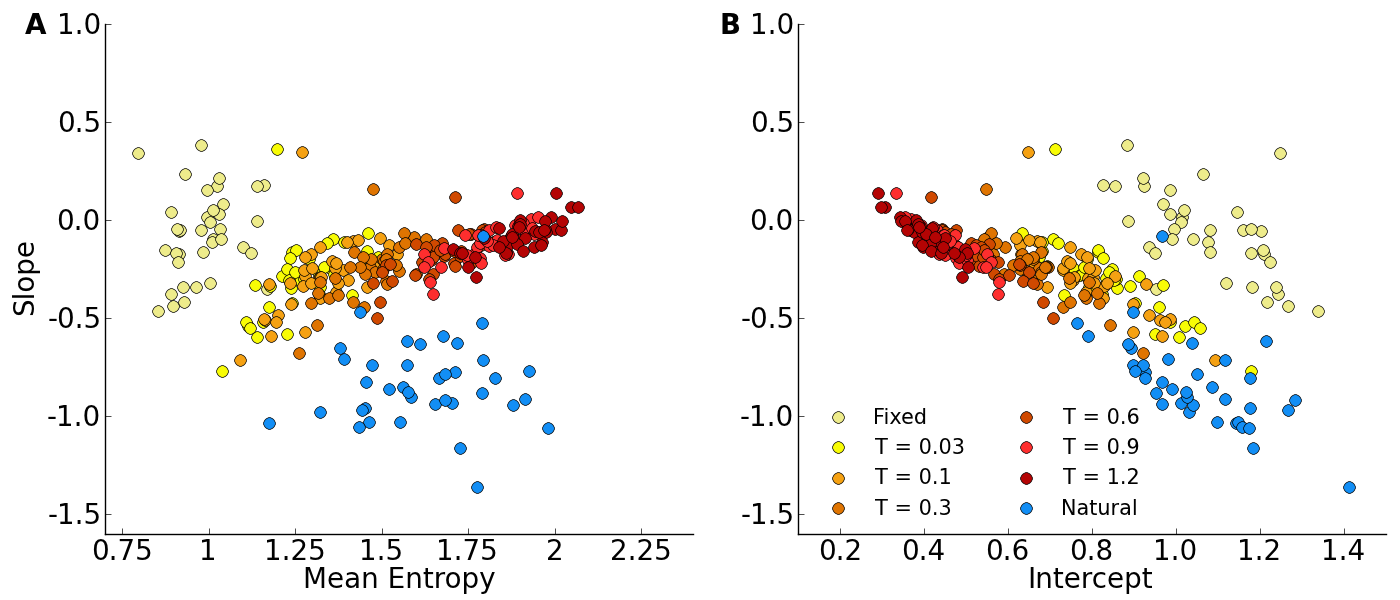
\includegraphics[width = 6in]{figures/Slope_Combination_Plot.png}}
\caption{Slopes calculated for 38 proteins. The slopes are calculated by fitting a linear function $\lambda=a\text{RSA}+b$ to these yeast proteins.  A) A plot of slope vs mean site entropy for 38 proteins. B) Intercepts vs Slopes for 38 proteins. Designed proteins have nonnegative slopes in contrast to the negative slope values found for natural proteins.  Natural proteins on average have a negative slope and a larger intercept when compared to designed proteins. Designed proteins on average have less negative slopes compared to natural proteins.}
\label{StructureFig3}
\end{figure}



%Figure 17
\begin{figure}[H]
\centering
%\centerline{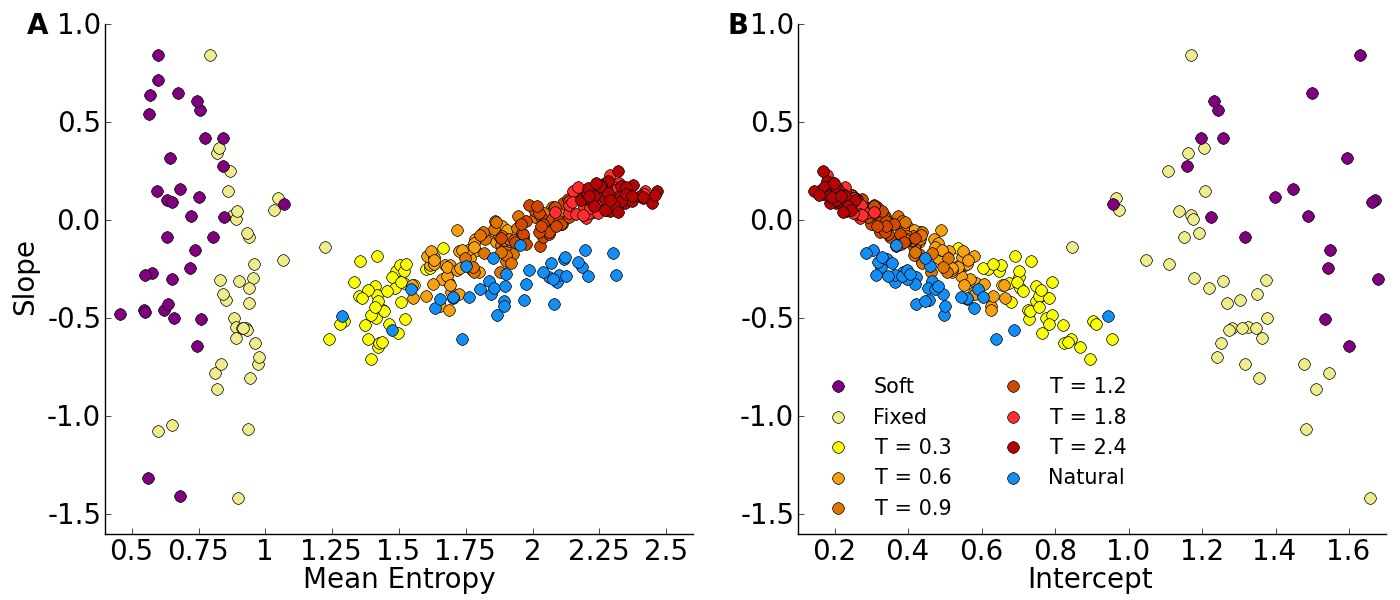
\includegraphics[width = 6in]{figures/Slope_Combination_Plot_Noah.png}}
\caption{Slopes calculated for 40 protein domains. The slopes are calculated by fitting a linear function $\lambda=a\text{RSA}+b$ to these yeast proteins.  A) A plot of slope vs mean site entropy for 40 protein domains. B) Intercepts vs Slopes for 40 protein domains. Designed proteins have nonnegative slopes in contrast to the negative slope values found for natural proteins.  Natural proteins on average have a negative slope and a larger intercept when compared to designed proteins.}
\label{NoahStructureFig3}
\end{figure}


%Figure 2
\begin{figure}[H]
\centering
%\centerline{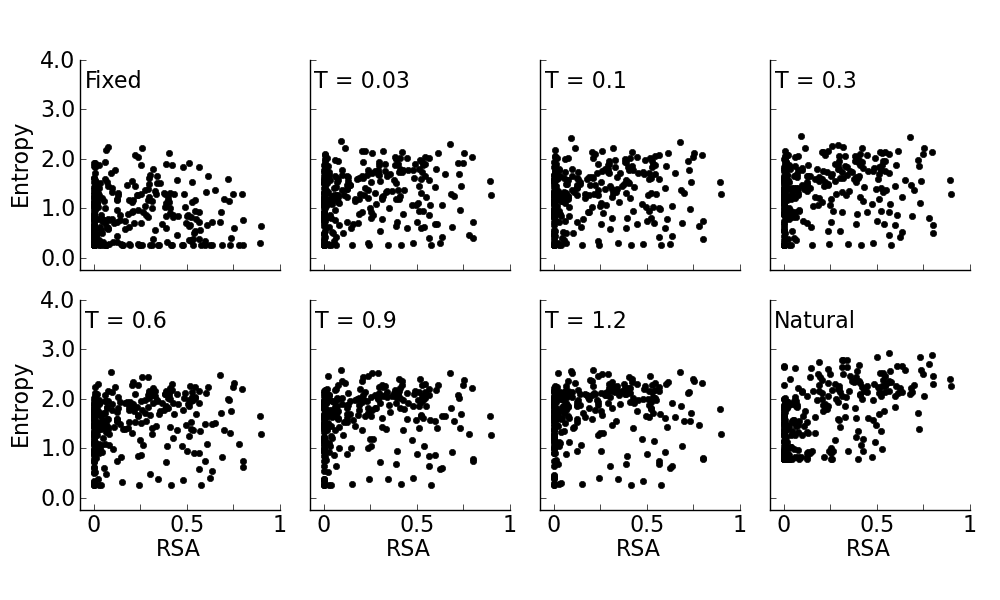
\includegraphics[width = 6.5in]{figures/RSA_vs_Entropy_1PV1_Combination_Plot.png}}
\caption{Entropy vs Relative Solvent Accessibility (RSA) for sites within the protein S - formylglutathione hydrolase (PDB: 1PV1, chain A). All RSA values are calculated from natural proteins. For most sites within the alignments created from the fixed backbone the entropy values are lower than they are in the natural proteins.  For designed proteins sites with backbone flexibility usually underestimate or overestimate entropy.}
\label{SiteVarFig2}
\end{figure}

%Figure 14
\begin{figure}[H]
%\centerline{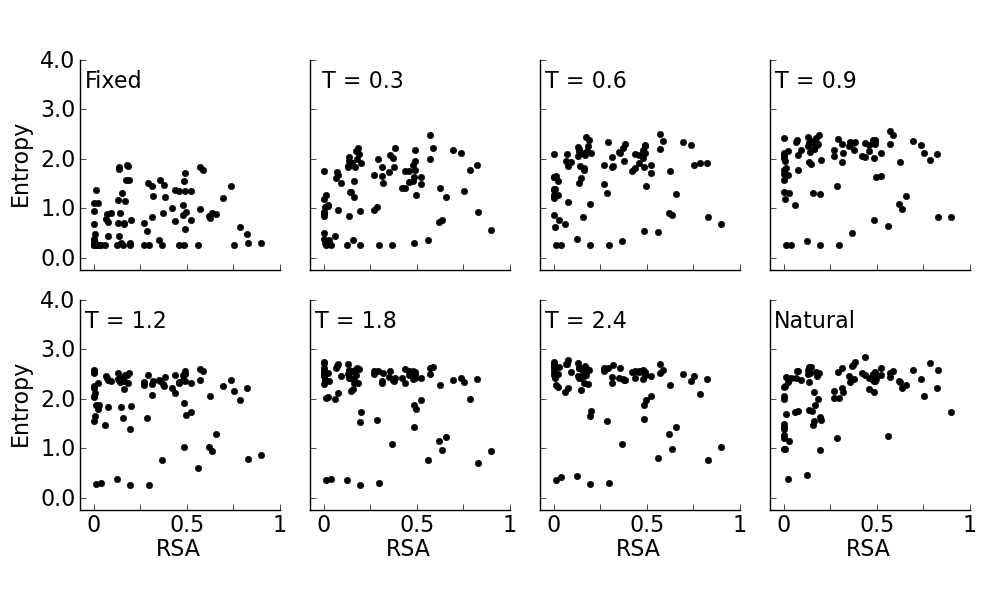
\includegraphics[width = 6.5in]{figures/RSA_vs_Entropy_2H3L_Combination_Plot_Noah.png}}
\caption{Entropy vs Relative Solvent Accessibility (RSA) for sites within the protein S - formylglutathione hydrolase (PDB: 2H3L, chain A). All RSA values are calculated from natural proteins. For most sites within the alignments created from the fixed backbone the entropy values are lower than they are in the natural proteins.}
\label{Entropy_Sites_Noah}
\end{figure}


%Figure 16
\begin{figure}[H]
%\centerline{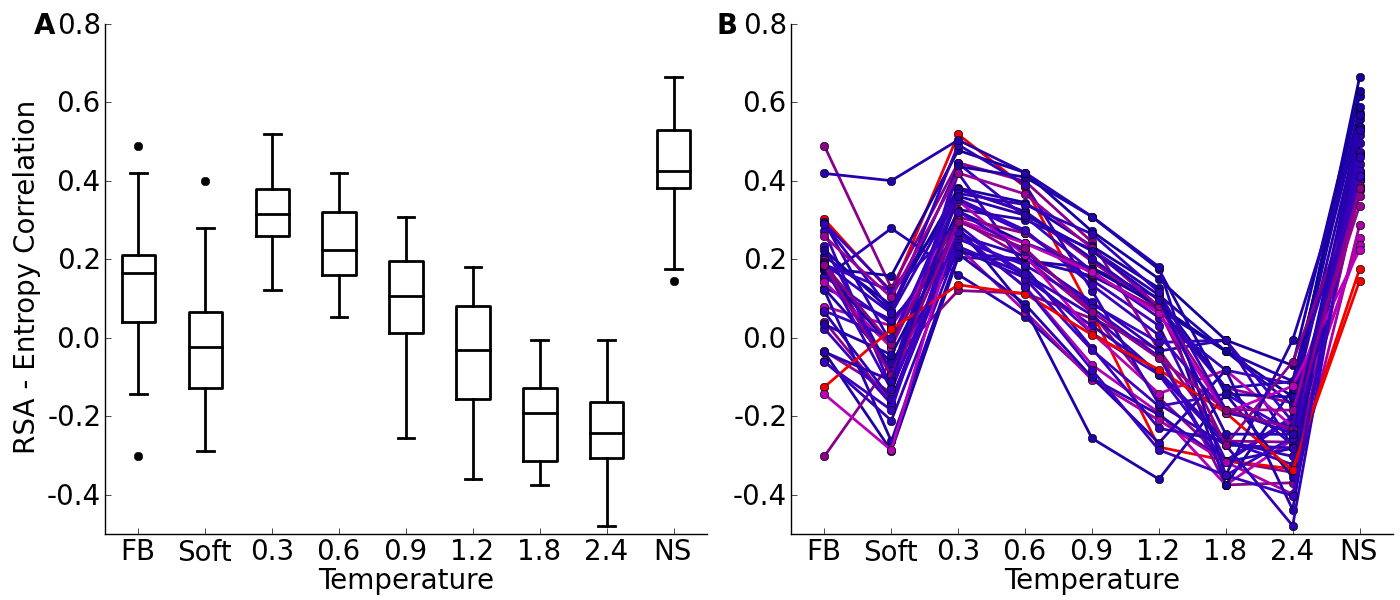
\includegraphics[width = 6in]{figures/Cor_Mean_Entropy_RSA_Combination_Plot_Noah.png}}
\caption{Correlation between Entropy and RSA for sites within proteins.  The temperatures represent alignments of designed proteins where an increased temperature relates to an increase level of backbone flexibility during the design process. A) Boxplots of the correlation between RSA and site entropy for various protein alignments. B) Lineplots of the correlation between RSA and site entropy for various protein alignments. The colors correspond to the value of the strength of the correlation between entropy and RSA at sites. }
\label{NoahStructureFig1}
\end{figure}

%Figure 21
\begin{figure}[H]
%\centering
%\centerline{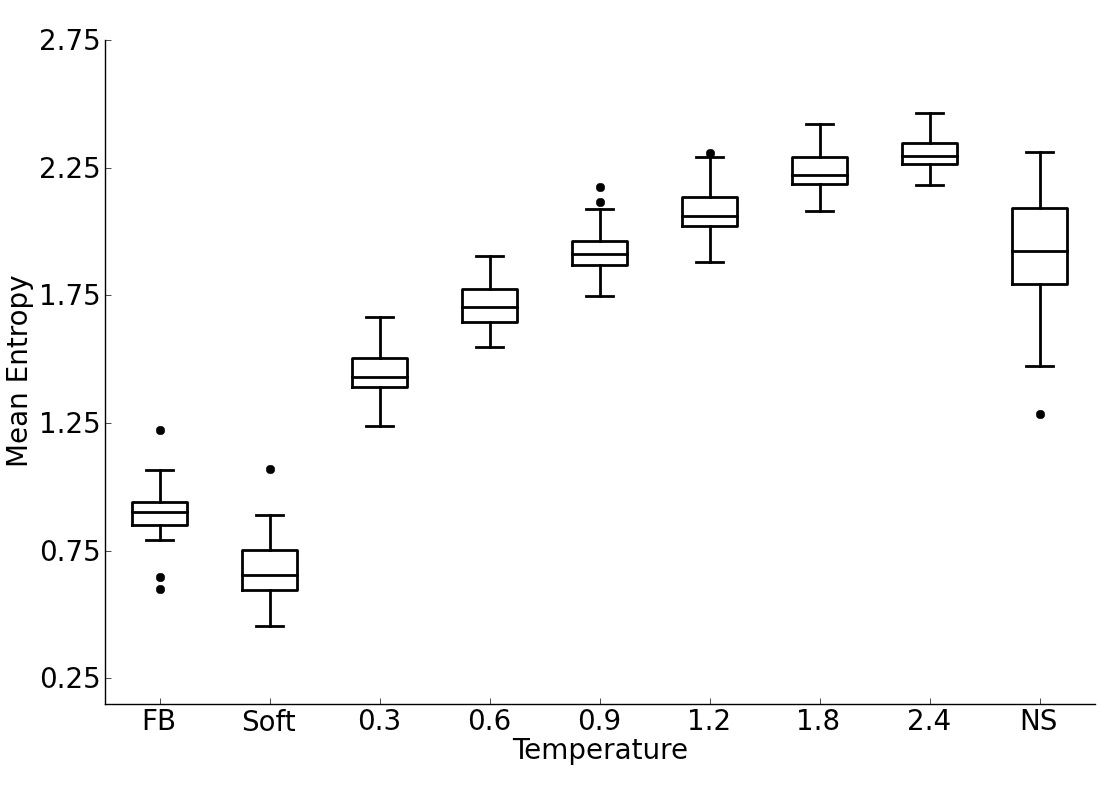
\includegraphics[width = 6in]{figures/Mean_Entropy_vs_Temp_Boxplot_Noah.png}}
\caption{Mean Entropy versus Temperature for sites within a series of designed proteins. The temperature refers to the temperature used during the designed process. Higher temperatures allowed for more backbone flexibility. FB and NS refer to the fixed backbone designed proteins and natural proteins respectively.  A site is categorized a buried site if it has an RSA of less than 0.05.}
\label{Mean_Entropy_Noah}
\end{figure}

%Figure 21
\begin{figure}[H]
%\centering
%\centerline{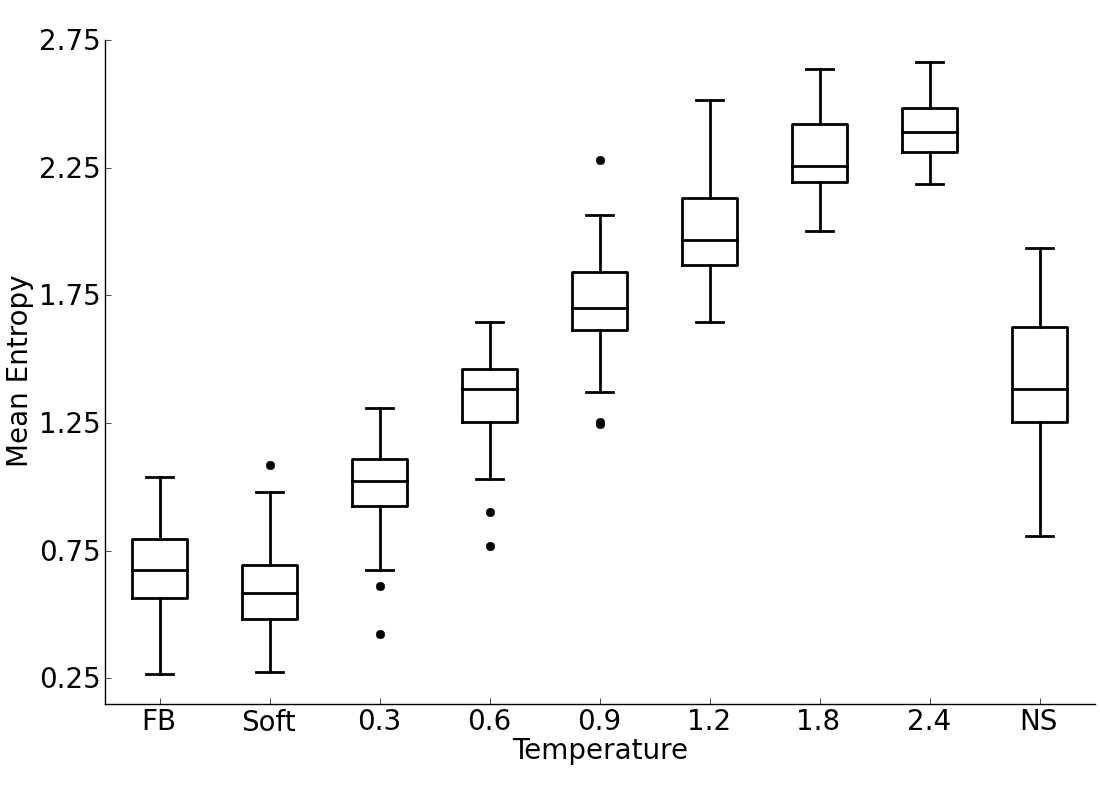
\includegraphics[width = 6in]{figures/Mean_Entropy_vs_Temp_Buried_Boxplot_Noah.png}}
\caption{Mean Entropy versus Temperature for buried sites within a series of designed proteins. The temperature refers to the temperature used during the designed process. Higher temperatures allowed for more backbone flexibility. FB and NS refer to the fixed backbone designed proteins and natural proteins respectively.  A site is categorized a buried site if it has an RSA of less than 0.05.}
\label{Buried_Entropy_Noah}
\end{figure}

%Figure 22
\begin{figure}[H]
%\centering
%\centerline{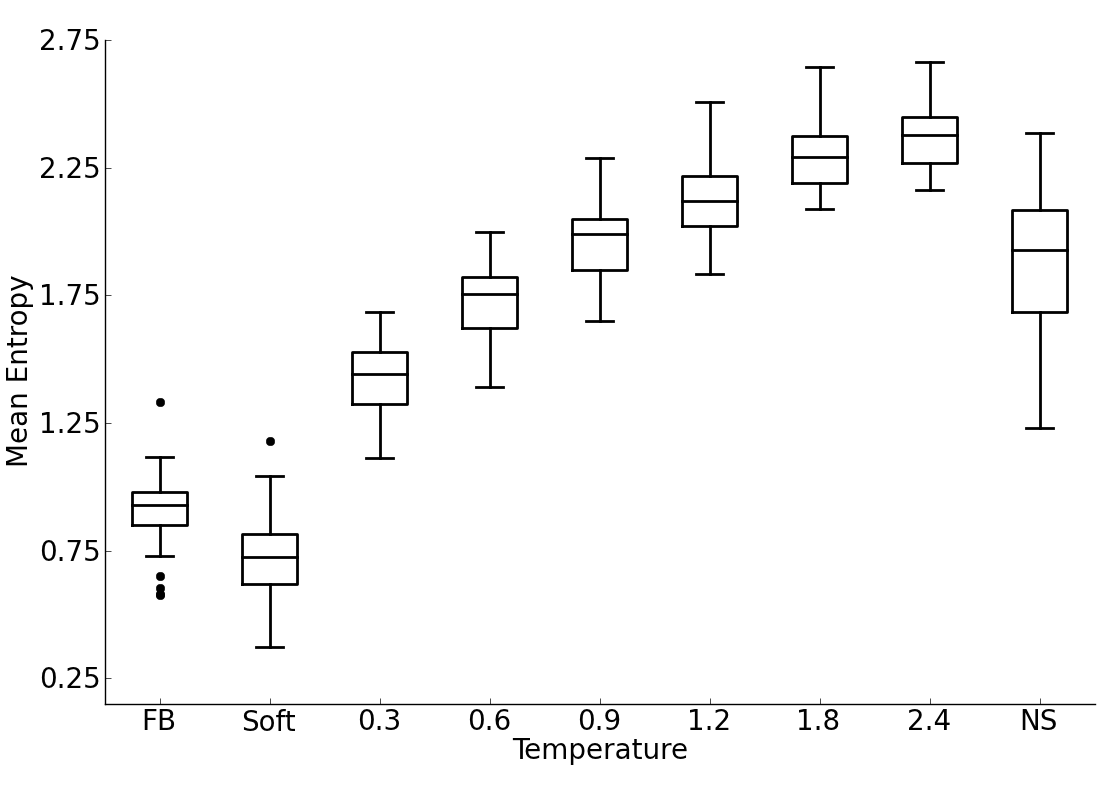
\includegraphics[width = 6in]{figures/Mean_Entropy_vs_Temp_Intermediate_Boxplot_Noah.png}}
\caption{Mean Entropy versus Temperature for partially buried sites within a series of designed proteins. The temperature refers to the temperature used during the designed process. Higher temperatures allowed for more backbone flexibility. A site is categorized as a partially buried site if it has a RSA of greater than or equal to 0.05 and less than or equal to 0.25. FB and NS refer to the fixed backbone designed proteins and natural proteins respectively.}
\label{Inter_Entropy_Noah}
\end{figure}

%Figure 23
\begin{figure}[H]
%\centering
%\centerline{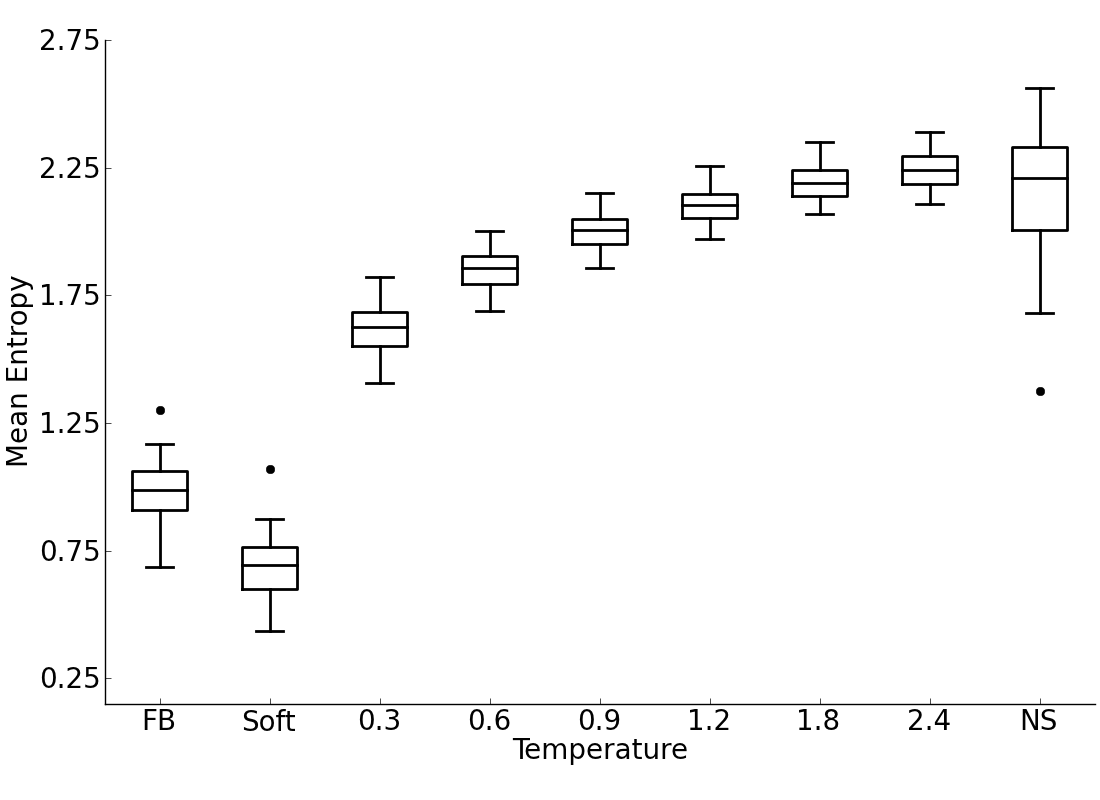
\includegraphics[width = 6in]{figures/Mean_Entropy_vs_Temp_Surface_Boxplot_Noah.png}}
\caption{Mean Entropy versus Temperature for exposed sites within series of 40 designed protein domains. The temperature refers to the temperature used during the designed process. Higher temperatures allowed for more backbone flexibility. A site is categorized as a surface site if it has a RSA of greater than 0.25. FB and NS refer to the fixed backbone designed proteins and natural proteins respectively.}
\label{Surface_Entropy_Noah}
\end{figure}

%Figure 24
\begin{figure}[H]
%\centering
%\centerline{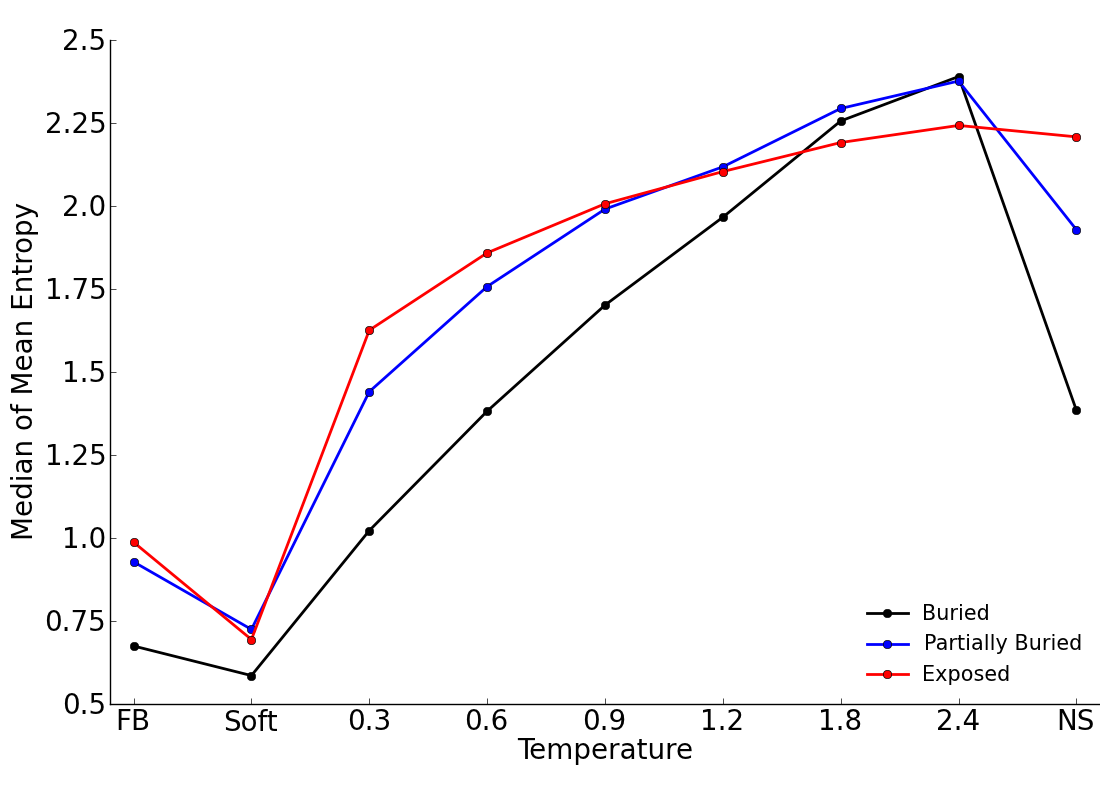
\includegraphics[width = 6in]{figures/Mean_Entropy_Position_Lineplot_Noah.png}}
\caption{Median of Mean Entropy versus Temperature sites within series of 40 designed protein domains.  Sites are classified as buried, partially buried, or exposed based on RSA magnitude. The temperature refers to the temperature used during the designed process. Higher temperatures allowed for more backbone flexibility. FB and NS refer to the fixed backbone designed proteins and natural proteins respectively.}
\label{Postion_Entropy_Noah}
\end{figure}

\end{document}